\chapter{Marco teórico de la propuesta}\label{chap:Conceptos}
En este capítulo se presenta todos los conceptos y técnicas usadas para el desarrollo de la propuesta desde las técnicas de detección usadas hasta el proceso de reconocimiento.

\section{Métodos de detección}

Es necesario resaltar la importancia de una detección adecuada para el reconocimiento ya que ambos son procesos muy relacionados entre sí. En esta sección se explican tres métodos de detección uno para encontrar rostros, otro para validar los rostros detectados y finalmente uno para encontrar puntos de dentro de los rostros.


\subsection{Detector de Viola-Jones}\label{scc:Viola}
El detector de Viola-Jones también conocido como \textit{Haar Detector} en implementaciones libres, se presenta en \cite{viola2001rapid} donde se hace uso de las características Haar (Figura \ref{im:Haar}) en una representación conocida como Imagen Integral, también se utiliza el Algoritmo Ada Boost y un clasificador en casada para completar el proceso de detección.

\begin{figure}[h]
\center
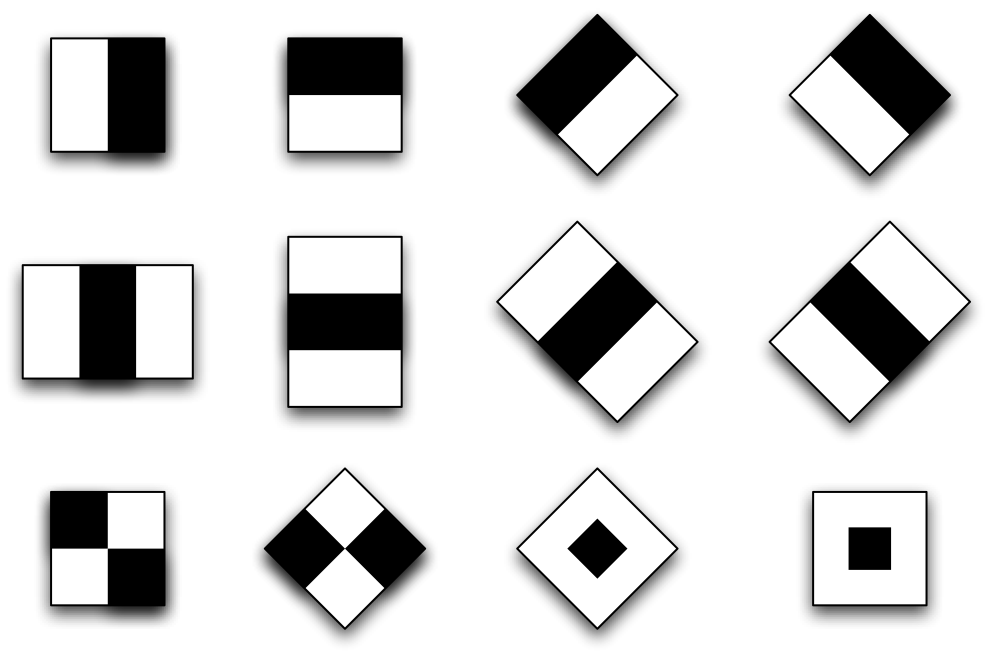
\includegraphics[scale=.5]{Haar}
\caption{Ejemplo de característica Haar, extraído de \cite{viola2001rapid}. Estos rectángulos pueden ser entendidos como rectángulos en los cuales son determinados como áreas de baja iluminación y otros como áreas de alta iluminación de esta manera podemos representar el contraste entre dos secciones de la imagen,}
\label{im:Haar}
\end{figure}

En \cite{viola2001rapid} se explica que el trabajo de detección se basa en tres conceptos:
\subsubsection{Imagen integral}
Usa un concepto parecido a una tabla de texturas donde tenemos en cada punto el valor de la suma de los pixeles de arriba y a la derecha de dicho punto. 

Esto permite el calculo rápido de valor de los pixeles para cualquier sección de la imagen, dicho valor nos ayuda a hacer un calculo rápido del contraste en cualquier sección, lo cual permite el calculo de cualquier característica Haar en tiempo constante.
\subsubsection{Algoritmo Ada Boost}
Debido a la existencia de un gran numero de características Haar, aproximadamente más de 45,000 no es posible usar todas en un proceso de clasificación, por lo que es necesario encontrar un conjunto pequeño de características que juntas formen un clasificador efectivo.

En \cite{viola2001rapid} se presenta una modificación al algoritmo Ada Boost para seleccionar las mejores características Haar y con ellas entrenar varios clasificadores débiles en términos de su tasa de aciertos, que en combinación permiten obtener un clasificador fuerte. De esta manera tener un clasificado robusto para el proceso de detección.
\subsubsection{Clasificador en casada}
La idea tras un clasificador en cascada es organizar todos los clasificadores débiles en un estilo en el cual estén uno detrás de otro como una cascada. Cuando se analiza una región esta pasa por el primer clasificador y sí el resultados es negativo se descarta, pero si resulta positivo pasa al siguiente clasificador hasta el final de la cascada y así sucesivamente de esta manera obtiene un solo clasificador, más robusto que los clasificadores que lo componen. Este proceso se puede apreciar en la Figura \ref{im:cascade}.

\begin{figure}[h]
\center
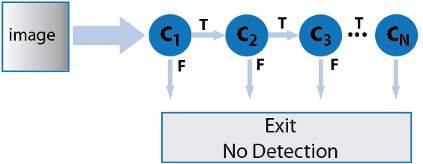
\includegraphics[scale=0.75]{cascadeClassifier}
\caption{Muestra del clasificador en cascada, donde una imagen es analizada por un clasificador tras otro desde el primero hasta el n-esimo si resulta la imagen positiva, extraído de \cite{viola2001rapid}.}
\label{im:cascade}
\end{figure}

El detector de Viola-Jones es ampliamente usado y reconocido como un detector que entrega una gran cantidad de verdaderos positivos (detecciones acertadas). Pero es necesario mencionar sus limitaciones y falencias, de la misma manera que entrega un gran porcentaje de verdaderos positivos también entrega falso  positivos (detecciones presentadas como verdaderas pero que no lo son) esto es debido a que el calculo de la imagen integral se hace en la escala de grises a veces alguna configuración de sombras producidas en la imagen genera la misma distribución de contrastes que un rostro humano.

Otro defecto es que solo detecta rostro de frente. No puede detectar otras posiciones del rostro humano simultáneamente. A pesar de estas deficiencia sigue siendo usado no solo para rostros sino para otro tipo de objetos ya que su mayor ventaja es que es entrenarle.

\subsection{Detector de \acf{HOG}}
Un detector de \acf{HOG} usa una combinación del descriptor de \ac{HOG} y un clasificador basado en \acf{SVM}, originalmente usado para detectar personas \cite{dalal2005histograms}, su uso se ha incrementado a varias situaciones, incluyendo la detección de rostros, a continuación exponemos las ideas detrás de este detector.
\subsubsection{Descriptor de \ac{HOG}}
Un descriptor de \ac{HOG} muestra el calculo de la gradiente de una imagen, la gradiente es cambio de la intensidad de la imagen en una cierta dirección, pudiendo ser representado como un vector que posee magnitud $g$ y dirección $\theta$, el calculo del gradiente en una imagen se hace por pixel y retorna la dirección del cambio y su magnitud, este proceso se observa en las siguientes ecuaciones:
\begin{equation}
dx=I(x+1,y)-I(x-1,y)
\end{equation}
\begin{equation}
dy=I(x,y+1)-I(x,y-1)
\end{equation}
\begin{equation}
\theta(x,y)=arctan\left(\frac{dy}{dx}\right)
\end{equation}
\begin{equation}
g(x,y)=\sqrt[2]{dx^2+dy^2}
\end{equation}

Donde $x$ y $y$ son las coordenadas de la imagen y la función $I(x,y)$ es el valor del pixel o intensidad en dichas coordenadas. Luego se divide la imagen en secciones iguales y en cada una de estas secciones se calcula un histograma de las orientaciones para conocer la orientación dominante de cada sección, de esta manera creamos un vector de características.

Con esta información se puede describir el contorno y forma de una figura, lo que es útil para realizar una clasificación.

\subsection{\acf{SVM}}
Un \ac{SVM} \cite{cortes1995support} es un clasificador lineal en el cual se intenta crear una linea divisoria entre las representación (vectores de características) de ejemplos positivos y negativos de un objeto determinado.

Esta basado en el aprendizaje estadístico para resolver problemas de clasificación de patrones. Los clasificadores lineales se caracterizan porque aprenden una función lineal para separar las clases. No se trata de una agrupación por similitudes, sin que existe una separación definida entre clases.

Dado un conjunto de ejemplos de entrenamiento (muestras) podemos etiquetar las clases y entrenar una SVM para construir un modelo que prediga la clase de una nueva muestra. Intuitivamente, una SVM es un modelo que representa a los puntos de muestra en el espacio, separando las clases por una linea representada por la función del clasificador. Cuando las nuevas muestras se ponen en correspondencia en función de su proximidad, pueden ser clasificadas a una u otra clase, dependiendo de la proximidad a cada una. Mas formalmente, la idea principal de SVM es construir un hiperplano o conjuntos de hiperplanos en un espacio de dimensionalidad muy alta como superficie de decisión, de tal forma que, el margen de separación entre ejemplos positivos y negativos sea el máximo. Una buena separación entre las clases permitirá una clasificación correcta. 

\ac{SVM} resulta ser un clasificador muy robusto y usado, el cual presenta varias modificaciones alrededor del estado del arte.


\subsection{\acf{CLNF}}
\ac{CLNF} es un método para encontrar puntos de interés en imágenes de rostros presentado en \cite{baltrusaitis2013constrained} e implementado para aplicaciones de video en \cite{Baltrusaitis2016} en la presentación de su framework ``Open Face'' para el tracking y detección de rostros, donde publica el código de su propuesta, \ac{CLNF} se basa en \ac{CLM}, por lo tanto empezamos con una explicación de \ac{CLM}.

\ac{CLM} es una forma para localizar un conjunto de puntos restringido por un modelo en una imagen, el proceso consiste en tomar una muestra de una área de la imagen donde se realizó una estimación inicial proyectarla a un marco de referencia. Por cada punto se genera una imagen de respuesta donde se le da una puntuación por tener el punto a localizar en cada pixel. Este puntaje es determinado a través de un detector local que evalúa el punto según un modelo de distribución de puntos en donde penaliza distribuciones complicadas y premia distribuciones simples y mas probables, de esta manera se evalúan todos los puntos en conjunto.

En \cite{baltrusaitis2013constrained} se propone el uso de redes neuronales para los detectores locales de los puntos, con lo cual logra una mejor determinación de puntos en relación con el resto de puntos detectados. Compara sus resultados con otras técnicas del estado del arte así mismo realiza pruebas con imágenes obtenidas de Internet que presentan condiciones no controladas.

\section{Técnicas de pre-procesamiento}
Como se puede observar en las secciones anteriores un problema en especial difícil es la iluminación, por lo que es necesario hablar sobre las técnicas de pre-procesamiento, se entiende como pre-procesamiento a las técnicas que modifican una imagen para acentuar alguna característica, estas serán usadas para afrontar dicho problema.

\subsection{Ecualización de histograma}
Las ecualización del histograma de una imagen es una transformación que pretende obtener para una imagen un histograma con una distribución uniforme. Es decir, que exista el mismo número de pixeles para cada nivel de gris del histograma de una imagen monocroma \cite{orlova2002image}.
La función de la ecualización es:
\begin{equation}
h(v)=Redondeo\Bigg(\frac{cdf(v)-cdf_{min}}{(M\times N)-cdf_{min}} \times (L-1)\Bigg)
\end{equation}
Donde $cdf_{min}$ es el mínimo valor no nulo de la función de distribución de acumulación. $M\times N$ es el numero de pixeles en la imagen y $L$ es el numero de niveles de la escala de gris.

\begin{figure}[h]
\center
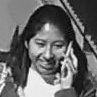
\includegraphics[scale=1]{face_original}
\hspace{1cm}
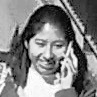
\includegraphics[scale=1]{face_he}
\caption{Ecualización de histograma - Izquierda: imagen en escala de Grises. Derecha: imagen ecualizada.}
\label{im:he}
\end{figure}


\subsection{Transformada de logaritmo}
La Transformada de logaritmo asigna un rango estrecho de valores (píxeles en escala de grises o un canal de un espacio de color) de un rango amplio de valores de entrada. La transformada de logaritmos es útil si se necesita expandir los valores de píxeles oscuros de una imagen mientras se comprime los valores altos \cite{thamiz2015liter}

\begin{equation}
\label{f_log}
s = c*log(1+ 256*r)
\end{equation}

Donde $r$ es la imagen de entrada, $c$ es una constante, $s$ es la imagen mejorada. Para la transformada de logaritmo se utilizo el valor de 20 para la constante $ c $. 

\begin{figure}[h]
\center
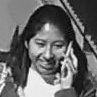
\includegraphics[scale=1]{face_original}
\hspace{1cm}
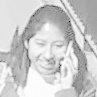
\includegraphics[scale=1]{face_log}
\caption{Transformada de logaritmo - Izquierda: imagen en escala de Grises. Derecha: imagen con Transformada de logaritmo.}
\label{im:log}
\end{figure}

\subsection{Transformada discreta de coseno}
La transformada Discreta de coseno (DCT por sus siglas en ingles) es utilizada especialmente en el procesamiento de señales e imágenes. DCT expresa en una secuencia finita de puntos, datos en términos de sumas de funciones de coseno en diferentes frecuencias. En el procesamiento de imágenes, la utilización de DCT ayuda a descomponer una imagen en frecuencias, donde usualmente los pequeños componentes de frecuencia altas pueden ser descartados. La ecuación en 2D está dada por la Ecuación. \ref{f_dct}
\cite{thamiz2015liter}\cite{vish2015ill}

\begin{equation}
	\label{f_dct}
	\resizebox{0.91\hsize}{!}{
		$ C(u,v) = \alpha(u)\alpha(v)\sum\limits_{x=0}^{N-1} \sum\limits_{y=0}^{N-1}f(x,y)cos\left[\frac{\pi(2x + 1)u}{2N}\right]cos\left[\frac{\pi(2y + 1)v}{2N}\right] $
	}
\end{equation}

Donde: $u$, $v$, $N$, $\alpha(u)$ y $\alpha(v)$ se definen de igual forma que la ecuación 1D. La ecuación inversa está definida por la Ecuación. \ref{f_idct}.

\begin{equation}
	\label{f_idct}
	\resizebox{0.91\hsize}{!}{
		$ f(x,y) = \sum\limits_{x=0}^{N-1}\sum\limits_{y=0}^{N-1} \alpha(u)\alpha(v)C(u,v)cos\left[\frac{\pi(2x + 1)u}{2N}\right]cos\left[\frac{\pi(2y + 1)v}{2N}\right]$
	}
\end{equation}

El resultado de la transformada de coseno, es una matriz de coeficientes positivos y negativos, los cuales representan la adición o resta de una determinada frecuencia para generar la imagen procesada por la transformada discreta de Coseno.

%parrafo para dar conclusion a la seccion
Se ha expuesto tres técnicas de pre-procesamiento que serán usadas en usadas en la propuesta del Capítulo \ref{chap:Propuesta}, todas abordan el problema de la iluminación de manera diferente, es necesario tener en cuenta que este problema ha sido tratado mucho en el estado del arte pero aun no se encuentra una técnica de mejora de iluminación sea robusta en cualquier escenario.

%En la siguiente sección se expone los métodos de detección usados como parte de nuestra propuesta. Se explica su funcionamiento y su posición en el estado del arte.


\section{\acf{EBGM}}\label{scc::EBGM}
%Después de haber tratado los métodos de pre-procesamiento, finalmente se expone las técnica de reconocimiento de rostro que en el Capítulo \ref{chap:Propuesta} se presenta una modificación.

\ac{EBGM} presentado en \cite{wiskott1997face} se basa en el concepto que las imágenes de los rostros reales tienen muchas características no lineales que no son abordadas por los métodos de reconocimiento holísticos, tales como variaciones en la iluminación, pose y expresión.
También se apoya en el argumento que las características visuales que se basan en Gabor Wavelet, han probado ser un buen modelo del procesamiento visual temprano en el cerebro, más precisamente células simples en la corteza visual primaria, por ello también se considera un algoritmo inspiración biológica.

Para ello, una transformación de Gabor wavelet crea una arquitectura de enlaces dinámicos que proyecta el rostro en una malla elástica que es conocida como Face Graph.
El Gabor Jet es un nodo en la malla elástica, el cual describe el comportamiento alrededor de un pixel. Esto es el resultado de la convolución de una imagen con varias máscaras de Gabor, el cual es usado para detectar formas y extraer características.

El reconocimiento esta basado en la similaridad de la respuesta mascara de Gabor a cada nodo. La dificultad con este método es el requerimiento de marcar puntos precisos en los rostros.

A continuación se explica en detalle su funcionamiento

\subsection{Gabor Wavelet}\label{sscc:GaborWavelet}
Las Gabor Wavelet son funciones que modifican las imágenes en el espacio de las frecuencias. El espacio de las frecuencia esta estrechamente relacionado al análisis de Fourier, por lo que es necesario hacer una breve descripción.

Una transformada de Fourier descompone una señal de tal manera que pueda ser representada como una combinación de sinusoidales. Cuando se procesa señales como lo pueden ser las imágenes, son representadas como una longitud de onda, ello es muy útil ya que revela información que no puede ser vista cuando observamos la imagen original.

Mientras una señal es un función en base al tiempo, la transformada de Fourier es una función en base a la frecuencia, se puede observar la transformada de Fourier en una dimensión en la siguiente ecuación:

\begin{equation}
F(x(t))(\omega)=\int_{-\infty }^{\infty } x(t)e^{-i\omega t}dt
\end{equation}

En la transformada de Fourier y en los Gabor Wavelet la función comprende una parte imaginaria y una real:

\begin{equation}
F(x(t))(\omega)=\int_{-\infty }^{\infty } x(t)cos(\omega t)dt - i\int_{-\infty }^{\infty } x(t)sen(\omega t)dt
\end{equation}

Cuando una transformada de Fourier se aplica una frecuencia en particular el resultado es un numero complejo que corresponde a la amplitud del coseno y del seno de la función original, en cada frecuencia hay un componte real y otro imaginario.

Las Gabor Wavelet son como la transformada de Fourier solo que tiene un alcance limitado, básicamente son una sinusoidal multiplicada por una Gaussiana.

Cuando una función es convolucionada con un Gabor Wavelet la información más cerca al centro de la campana de la Gaussiana es la que es tomada en cuenta mientras la más lejana es ignorada.

La ecuación de una de una Gabor Wavelet es la siguiente:
\begin{equation}
W(t,t_0,\omega)=e^{-\sigma(t-t_0)^2} e^{--i\omega(t-t_0)}
\end{equation}
y su convolucion es:
\begin{equation}
C(x(t))(t_0,\omega)=\int_{-\infty}^{\infty}x(t)W(t,t_0,\omega)dt
\end{equation}

De la misma manera que Fourier produce una resultado complejo un Gabor Wavelet produce:
\begin{equation}
C(x(t))(t_0,\omega)=a_{real}+ia_{imag}
\label{ec:ConvolucionWavelet}
\end{equation}

Mientras las ecuaciones presentadas hasta ahora trabajan en una dimensión es necesario presentar una forma en la que se pueda trabajar en dos dimensiones, esta es la representación del Gabor Wavelet como mascara para una convoluciónn en imágenes.

La Ecuación \ref{GaborWavelet} define como crear una máscara de Gabor donde $x, y$ son las posiciones en la mascara, para cualquier tamaño de mascara.
%El Gabor Jet es un nodo en la malla elástica, el cual describe el comportamiento alrededor de un pixel. Esto es el resultado de la convolución de un pixel de la imagen con varios Gabor wavelet o máscaras de Gabor, los cuales son usados para detectar formas y extraer características.

\begin{equation}
W(x,y,\theta,\lambda, \phi, \sigma, \gamma )=e^{-\frac{x'^2+\gamma y'^2}{2 \sigma^2}}cos(2\pi \frac{x'}{\lambda}+\phi) 
\label{GaborWavelet}
\end{equation}
\begin{equation*}
x'=cos\theta+ysin\theta   
\label{GaborWaveletx}
\end{equation*}
\begin{equation*}
y'=-x sin\theta+ycos\theta
\label{GaborWavelety}
\end{equation*}
Los parámetros usados para la construcción de los Gabor wavelet son los mismo que se utilizan en la implementación de \cite{bolme2003elastic}, a continuación los explicamos brevemente:
\begin{itemize}
\item $\theta$ especifica la orientación del Gabor Wavelet.\\
Siendo $\theta \in \left\{0,\pi/8,2\pi/8,3\pi/8,4\pi/8,5\pi/8,6\pi/8,7\pi/8 \right\}$
\item $\lambda$ especifica el ancho de onda de la función seno, empieza con 4 pixeles y aumenta en medias octavas siendo $\lambda \in \left\{4,4\sqrt{2},8,8\sqrt{2},16\right\} $
\item $\phi$ especifica la fase de la función seno, pudiendo ser par e impar que representa la parte imaginaria y la parte real del wavelet respectivamente.
Siendo $\left\{0,\pi/2\right\}$
\item $\delta$ especifica el radio de la Gaussiana. En este caso $\delta=\lambda$.
\item $\gamma$ especifica el ratio de aspecto de la Gaussiana. Este parámetro es incluido para que el Wavelet se aproxime a ciertos modelos biológicos. Siendo $\gamma=1$.
\end{itemize}


De esta manera podemos crear varios tamaños de máscaras que en la configuración original son $N \in \left\{25, 37, 51, 71, 101 \right\}$. Dando 80 configuraciones de Gabor wavelet y siendo efectivas 40 máscaras por punto, debido a que existe una mascara que extraer la parte imaginara y otra la parte real del Wavelet.
%buscar imagen de las mascaras

Al conjunto coeficientes (reales e imaginarios) producidos por estas mascaras de Gabor son llamados Gabor Jet que son el corazón de todo el proceso de reconocimiento de \ac{EBGM}.

A continuación se explica como es el proceso por el cual \ac{EBGM} determina en que puntos de una imagen va extraer características. A estos punto se les conocen como puntos fiduciales.

\subsection{Localización de puntos fiduciales}
Como se menciona en la sección anterior la convolución del conjunto de mascaras de Gabor sobre un punto produce un Gabor Jet que es un conjunto de coeficientes.

\begin{figure}[h]
\center
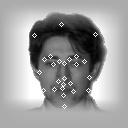
\includegraphics[scale=1.5]{Points}
\caption{Muestra de los puntos fiduciales elegidos en \ac{EBGM}\cite{bolme2003elastic}, en cada punto se realiza 40 convoluciones con máscaras de Gabor para crear un Gabor Jet por punto}
\label{im:puntos}
\end{figure}

Siguiendo el trabajo de \cite{wiskott1997face}, Bolme realiza una implementación de código libre de todo el algoritmo y da un mayor detalle de su funcionamiento, listando que puntos de interés debemos encontrar en una imagen. Estos puntos son conocidos como puntos fiduciales, en el Cuadro \ref{ta:PuntosFiduciales} se puede observar una lista de ellos, y en la Figura \ref{im:puntos} se puede ver su localización.

\begin{table}[h]
\centering
\caption{Lista de puntos fiduciales presentada en \cite{bolme2003elastic}}
\label{ta:PuntosFiduciales}
\begin{tabular}{|l|l|}
\hline
1. Ojo izquierdo                          & 2. Ojo derecho                          \\ \hline
3. Centro del puente de la nariz          & 4. Pico de la ceja izquierda            \\ \hline
5. Pico de la ceja derecha                & 6. Interior de la ceja izquierda        \\ \hline
7. Interior de la ceja derecha            & 8. Exterior de la ceja izquierda        \\ \hline
9. Exterior de la ceja derecha            & 10. Centro de la punta de la nariz      \\ \hline
11. Centro de la base de la nariz         & 12. Izquierda de la base de la nariz    \\ \hline
13. Derecha de la base de la nariz        & 14. Centro parte superior boca          \\ \hline
15. Centro parte inferior boca            & 16. Esquina izquierda de la boca        \\ \hline
17. Esquina derecha de la boca            & 18. Parte central del tope de la cabeza \\ \hline
19. Parte izquierda del tope de la cabeza & 20. Parte derecha del tope de la cabeza \\ \hline
21. Costado izquierdo del rostro          & 22. Costado derecho del rostro          \\ \hline
23. Centro de la barbilla                 & 24. Quijada izquierda                   \\ \hline
25. Quijada derecha                       &                                         \\ \hline
\end{tabular}
\end{table}

El método por el cual \ac{EBGM} encuentra los puntos fiduciales es a través del uso de moldes, imágenes en  las cuales los puntos han sido encontrados manualmente. En los trabajos de \cite{wiskott1997face} y \cite{bolme2003elastic} utilizan 70 imágenes normalizada a un mismo tamaño y donde las coordenadas de los ojos son las mismas.

Sobre cada imagen de molde y en cada punto marcado se realiza las convoluciones de las mascaras de Gabor para producir un Gabor Jet, de esta manera todos los puntos en todas las imágenes tienen un Gabor Jet. Finalmente todos los Gabor de un punto, por ejemplo el ojo izquierdo, son reunidos en un solo grafo conocido como Bucnh Graph que contiene todos los Gabor Jet de los modelos.

De esta manera se obtiene un modelo general con información de todos los modelos, también contiene la información de coordenada de cada punto en cada modelo y un punto de coordenada promedio.

Para reconocer una nueva imagen se realiza una normalización de tamaño y una traslación coordenadas de los ojos a coordenadas preestablecidas a través de una transformación matricial. Mediante un alineamiento entre las coordenadas normalizadas de los ojos y las coordenadas de los ojos del Bunch Graph se encuentran el resto de los puntos fiduciales en la imagen usando la información de coordenada promedio almacenada en el Bunch Graph. Finalmente se encuentra la posición final del punto usando como referencia el Gabor Jet con mayor similaridad en el Bunch Graph

Según \cite{bolme2003elastic} y \cite{wiskott1997face}, y como se menciona en la sección anterior el resultado de una transformada de Fourier en una función y en una frecuencia determinada es un numero complejo, que tiene una correspondencia en amplitud en términos de senos y cosenos que pueden ser representada como una coordenada polar.
\begin{equation}
x_{\omega}(t)=a_{\omega,r}cos(t)+a_{\omega,i}sin(t)= a cos(t+\phi).
\label{ec:CorrepondeciaAPolar}
\end{equation}
Es posible representar las suma de las sinusoidales como una función coseno dándole una amplitud y fase especifica.
Esto sucede cuando las sinusoidales son multiplicadas por una Gaussiana como se observa en la Ecuación \ref{ec:ConvolucionWavelet} y según lo visto en la Ecuación \ref{ec:CorrepondeciaAPolar} se puede representar los coeficientes complejos del resultado de las convoluciones como coordenadas polares de magnitud $a$ y un angulo $\phi$
\begin{equation}
a_{real} = a cos\phi 
\end{equation}
\begin{equation}
 a_{imag} = a sen\phi 
\end{equation}
y podemos halla $a$ y $\phi$ mediante:
\begin{equation}
a = \sqrt{a^2_{real}+a^2_{imag}}
\end{equation}
\begin{equation}
\phi=\left\{\begin{matrix}
arctan(a_{imag}/a_{real}) & \textrm{si } a_{real}>0 \\ 
\pi+arctan(a_{imag}/a_{real}) & \textrm{si } a_{real}<0 \\ 
\pi/2 & \textrm{si } a_{real}=0 \textrm{ y } a_{imag}>= 0 \\ 
-\pi/2 & \textrm{si } a_{real}=0 \textrm{ y } a_{imag}<0
\end{matrix}\right.
\end{equation}
Gracias a esta transformación a coordenadas polares podemos representar la información compleja del resultado de la convolucion de una mascar de Gabor. 
%Existe una relación entre el desplazamiento de tiempo en frecuencia y el angulo de la fase del coeficiente. Sí los coeficientes de dos puntos separados por un pequeño desplazamiento son calculados, la diferencia entre el angulo de la fase de dichos puntos debe ser proporcional al desplazamiento entre dichos puntos.

%De esta manera solo se convolusiona el punto una vez, cuando se hace la estimacion inicial y se elige el Gabor Jet mas parecido del Bunch Graph y sobre el se calcula el desplazamiento así para calcular la posición final del punto fiducial, este proceso es el que le da el nombre de \textit{elastic} a \ac{EBGM}.

Cabe mencionar que la mayor debilidad del algoritmo yace en este proceso ya que si el alineamiento del grafo falla por culpa de un error en las coordenadas de los ojos el resto de las estimaciones iniciales falla. % y a pesar de tener una función para el calculo de desplazamiento está limitada a pequeños desplazamientos y búsquedas locales ya que no es practico que haga las estimación a lo largo de grande porciones de la imagen.
Otra dificultad que presenta es la dependencia a sus modelos, esto quiere decir que por ejemplo si entre sus modelos no se encuentra alguien con barba cuando se intente encontrar puntos en nueva imagen de una persona con barba no va existir ningún Gabor Jet en el Bunch Graph que sea una buena referencia para el ajuste de la posición final del punto.

Finalmente es necesario contar con las coordenadas de ojos de antemano, este hecho por simple que parezca es una de las limitaciones para que \ac{EBGM} se pueda usar en un sistema de reconocimiento de rostro automatizado sobre todo en vídeo vigilancia donde encontrar ojos es difícil.

\subsection{Face Graph}
Una vez hallada la posición final de los puntos se extrae los coeficientes finales (la representación en coordenadas polares de la convolucion) para los Gabor Jet donde se almacenan una estructura que se conoce como Face Graph. A pesar que en la literatura se representa como un grafo , Figura \ref{im:FaceGraph} , Un Face Graph en realidad es un vector de características.
\begin{figure}[h]
\center
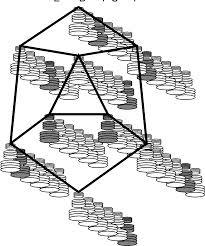
\includegraphics[scale=0.9]{BunchGraph}
\caption{Representación de Face Graph presentada en \cite{wiskott1997face} }
\label{im:FaceGraph}
\end{figure}

Al final solo se hace una comparación punto a punto entre dos Face Graph para el proceso de reconocimiento.

\subsection{Función de similitud}
El proceso de reconocimiento se lleva a cabo mediante una función de similitud que compara cuan iguales son dos Face Graph, dicha función se expresa de la siguiente forma:
\begin{equation}
\label{FaceGraphSimiFunc}
L_{jet}(G,G')=\frac{1}{N}\sum_{i=0}^{N}S(J_{i},J'_{i})
\end{equation}
Donde $N$ es el numero de puntos fiduciales y $J_i,J'_i$ son los i-ésimos Gabor Jet que pertenecen respectivamente a los Face Graph $G,G'$ que van a ser comparados.

La función de similitud entre dos Gabor Jet es la siguiente:
\begin{equation}
\label{GaborJetSimiFunc}
S(J,J')=\frac{\sum_{j=1}^{N}a_j a'_jcos(\phi_j-\phi'_j)}{\sqrt{\sum_{j=1}^{N}a_j^2 \sum_{j=1}^{N}{a'}_j^2}}
\end{equation}

%escribir un parrafo sobre la comparacion de givens
Después de explicar el funcionamiento de \ac{EBGM} es necesario mencionar las situaciones donde tiene problemas para funcionar, según \cite{givens2004features} en su estudio comparativo con \ac{PCA} donde explica varias pruebas. Cuando hay cambios bruscos de expresión, cambio de los ojos y boca, y ojos cerrados son las situaciones en las cuales \ac{EBGM} tiene problemas para realizar el reconocimiento, finalmente concluye que dichos problemas tienen en parte relación con el hecho que se necesita las coordenadas de los ojos para empezar el reconocimiento y las dificultades relacionadas para encontrar dichas posiciones afectan el desempeño del algoritmo.

%parrafo para terminar la seccion
En esta sección se explicó el funcionamiento de \ac{EBGM} que extrae característica de partes bien definidas del rostros, que también son conocidas como características biométricas.

%En un contexto de vídeo vigilancia no solo hace falta elegir un método de reconocimiento de rostros, también en necesario establecer que características van a ser medidas y como ellas van a ser identificadas por ello es necesario explicar el concepto de reconocimiento biométrico.

\section{Consideraciones finales}
En este capítulo se ha expuesto todos los métodos que interviene en alguna u otra forma en la propuesta, se ha presentado una introducción a cada una de ellos.

Es necesario resaltar que \ac{EBGM} es un método de reconocimiento biométrico, que se refiere a una forma de reconocimiento basado en un vector de características que derivan mayormente de características biológicas, se considera mucho mas confiable que otros métodos de reconocimiento que usan claves, contraseñas, tarjetas, etc \cite{alice2003biometric}. Esto se debe a cumple con los requerimientos necesarios para ser considerado como tal siendo estos los siguientes:

\begin{itemize}
\item Universalidad.- Toda persona debe tener dicha característica.
\item Distintividad.- Cualquier par de personas debe ser diferente en términos de dicha característica
\item Permanencia.-La característica debe ser lo suficientemente invariable a lo largo del tiempo para que pueda ser usada como criterio de comparación.
\item Medible.-La característica debe ser cuantitativamente mensurable.
\end{itemize}

Por ello es adecuado su uso para un escenario de vídeo vigilancia en el cual se aplica la propuesta presentada en el siguiente capítulo.

